\documentclass[conference]{IEEEtran} 
\IEEEoverridecommandlockouts
\usepackage{cite}
\usepackage{amsmath,amssymb,amsfonts}
\usepackage{algorithmic}
\usepackage{flafter}
\usepackage{graphicx}
\usepackage{textcomp}
\usepackage{xcolor}
\graphicspath{ {imagenes/} }

\begin{document}

\title{Actividad 1.1 \\ Sistemas de Numeración }

\author{\IEEEauthorblockN{Ricardo David López Arellano}
\IEEEauthorblockA{\textit{Departamento de Ingeniería en Computación} \\
\textit{CUCEI}\\
Universidad de Guadalajara\\
ricardo.lopez1361@alumnos.udg.mx} }
\onecolumn

\maketitle

\section{Originalidad}
Me comprometo a producir trabajo académico íntegro, lo que significa un trabajo que se adhiere a los estándares intelectuales y académicos de atribución exacta de las fuentes, uso y recolección de datos apropiados, y transparencia en el reconocimiento de las contribuciones de las ideas, descubrimientos, interpretaciones y conclusiones de otros.
Acepto que la trampa en los exámenes, el plagio o la fraudulenta representación de las ideas o lenguaje de otros como propio, la falsificación de datos o cualquier otra instancia de deshonestidad académica, violan los estándares de LA MATERIA, así como los estándares del mundo en general en el campo del conocimiento y las relaciones.

\section{Introducción}
\begin{center}
Un sistema de numeración es un conjunto de símbolos y reglas de generación que permiten construir todos los números válidos.
\end{center}

\section{Objetivos de la actividad}
\begin{center}
• Implementar dos funciones para la conversión de los sistemas de numeración.
\end{center}

\section{Metodología}
• Diseña e implementa dos funciones para la conversión entre sistemas de numeración en lenguaje C, donde la declaración de dichas funciones es la siguiente: \\
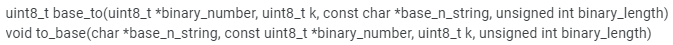
\includegraphics{e1} \\

Siendo baseto una función que permite convertir una cadena de texto que contiene los dígitos de la base B = 2 a la 'k' (k es el número de bits: 1 a 6) a un número binario de longitud máxima, y regresa el número de bytes que contiene el número binario. Mientras que tobase es una función que permite convertir un número binario binarynumber de longitud binarylength a una cadena de texto basestring, la cual contiene los dígitos de la base B = 2 a la 'k' (k es el número de bits: 1 a 6).

\section{Contenido}
\subsection{Código:}
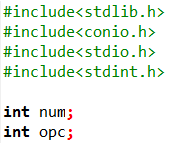
\includegraphics{e2} \\
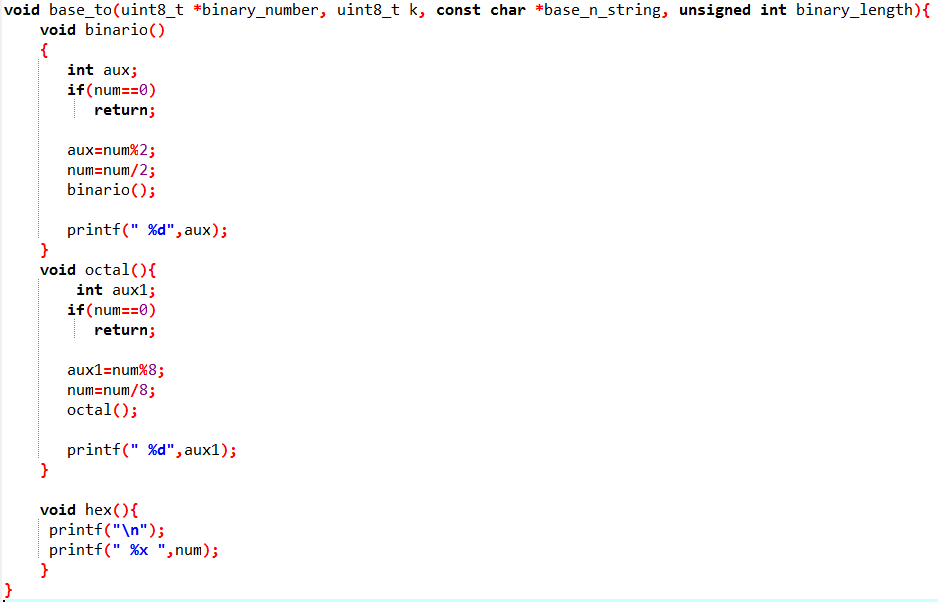
\includegraphics{e3} \\
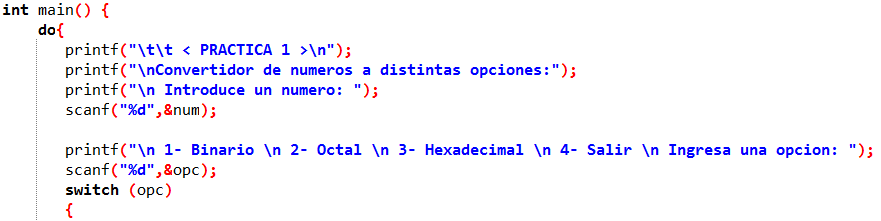
\includegraphics{e4} \\
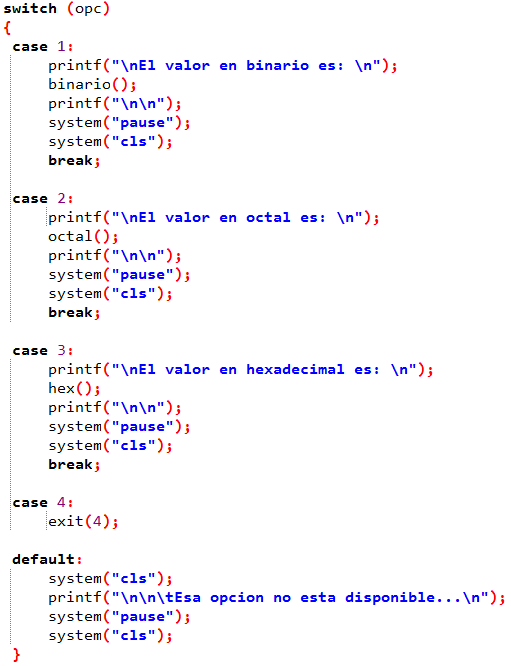
\includegraphics{e5} \\
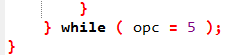
\includegraphics{e6} \\

\section{Resultados}
	\begin{center}
	Estos fueron los resultados de mi corrida de mi programa: \\
	\textbf{Respuesta: } \\
	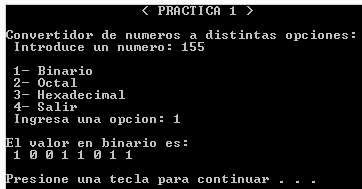
\includegraphics{e7} \\
	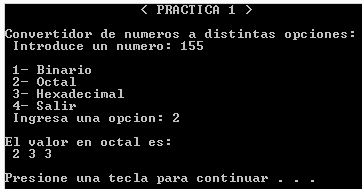
\includegraphics{e8} \\
	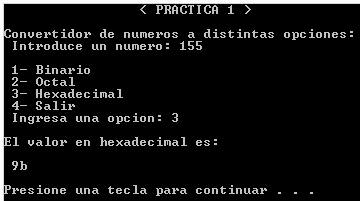
\includegraphics{e9} \\
	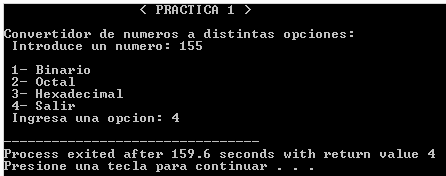
\includegraphics{e10} \\
	\end{center}

\section{Conclusiones}  
En conclusión a esta tarea puedo decir que al principios de semestre no la realice ya que no puede descargar Latex para hacer el reporte y hacer el reporte era prácticamente el 50 de calificación de la tarea, ya después si lo logré instalar pero como seguimos avanzando con más trabajos olvidé por completo realizar la tarea, espero y puedo valer aunque sea un poco para subir mi calificación final. De ante mano muchas gracias por su tiempo profesor, me gustó su forma de enseñar ojalá pueda volver a encontrármelo en otra materia.

\section*{Agradecimientos}
Quiero hacer agradecimiento a mi profesor por explicarme cuando tenia dudas sobre cómo hacer las conversiones a principios de semestre ya que eso fue la base para poder realizar éste programa y a mis padres en apoyarme cuando los necesito.

\begin{thebibliography}{00}
\bibitem{Alvarez2022} Becerra Alvarez, E. C. (2022, 4 octubre). https://drive.google.com/file/d/1mNTais1aV0h3mnluL8FKdbOD-9R0n0t/view

\end{thebibliography}

\end{document}